\documentclass[]{article}
\usepackage{lmodern}
\usepackage{amssymb,amsmath}
\usepackage{ifxetex,ifluatex}
\usepackage{fixltx2e} % provides \textsubscript
\ifnum 0\ifxetex 1\fi\ifluatex 1\fi=0 % if pdftex
  \usepackage[T1]{fontenc}
  \usepackage[utf8]{inputenc}
\else % if luatex or xelatex
  \ifxetex
    \usepackage{mathspec}
  \else
    \usepackage{fontspec}
  \fi
  \defaultfontfeatures{Ligatures=TeX,Scale=MatchLowercase}
\fi
% use upquote if available, for straight quotes in verbatim environments
\IfFileExists{upquote.sty}{\usepackage{upquote}}{}
% use microtype if available
\IfFileExists{microtype.sty}{%
\usepackage{microtype}
\UseMicrotypeSet[protrusion]{basicmath} % disable protrusion for tt fonts
}{}
\usepackage[margin=1in]{geometry}
\usepackage{hyperref}
\hypersetup{unicode=true,
            pdftitle={Mentor Work Sample for Statistical Inference: Simulations and Hypothesis Testing with R},
            pdfauthor={Kunyu Quinn He},
            pdfborder={0 0 0},
            breaklinks=true}
\urlstyle{same}  % don't use monospace font for urls
\usepackage{color}
\usepackage{fancyvrb}
\newcommand{\VerbBar}{|}
\newcommand{\VERB}{\Verb[commandchars=\\\{\}]}
\DefineVerbatimEnvironment{Highlighting}{Verbatim}{commandchars=\\\{\}}
% Add ',fontsize=\small' for more characters per line
\usepackage{framed}
\definecolor{shadecolor}{RGB}{248,248,248}
\newenvironment{Shaded}{\begin{snugshade}}{\end{snugshade}}
\newcommand{\KeywordTok}[1]{\textcolor[rgb]{0.13,0.29,0.53}{\textbf{#1}}}
\newcommand{\DataTypeTok}[1]{\textcolor[rgb]{0.13,0.29,0.53}{#1}}
\newcommand{\DecValTok}[1]{\textcolor[rgb]{0.00,0.00,0.81}{#1}}
\newcommand{\BaseNTok}[1]{\textcolor[rgb]{0.00,0.00,0.81}{#1}}
\newcommand{\FloatTok}[1]{\textcolor[rgb]{0.00,0.00,0.81}{#1}}
\newcommand{\ConstantTok}[1]{\textcolor[rgb]{0.00,0.00,0.00}{#1}}
\newcommand{\CharTok}[1]{\textcolor[rgb]{0.31,0.60,0.02}{#1}}
\newcommand{\SpecialCharTok}[1]{\textcolor[rgb]{0.00,0.00,0.00}{#1}}
\newcommand{\StringTok}[1]{\textcolor[rgb]{0.31,0.60,0.02}{#1}}
\newcommand{\VerbatimStringTok}[1]{\textcolor[rgb]{0.31,0.60,0.02}{#1}}
\newcommand{\SpecialStringTok}[1]{\textcolor[rgb]{0.31,0.60,0.02}{#1}}
\newcommand{\ImportTok}[1]{#1}
\newcommand{\CommentTok}[1]{\textcolor[rgb]{0.56,0.35,0.01}{\textit{#1}}}
\newcommand{\DocumentationTok}[1]{\textcolor[rgb]{0.56,0.35,0.01}{\textbf{\textit{#1}}}}
\newcommand{\AnnotationTok}[1]{\textcolor[rgb]{0.56,0.35,0.01}{\textbf{\textit{#1}}}}
\newcommand{\CommentVarTok}[1]{\textcolor[rgb]{0.56,0.35,0.01}{\textbf{\textit{#1}}}}
\newcommand{\OtherTok}[1]{\textcolor[rgb]{0.56,0.35,0.01}{#1}}
\newcommand{\FunctionTok}[1]{\textcolor[rgb]{0.00,0.00,0.00}{#1}}
\newcommand{\VariableTok}[1]{\textcolor[rgb]{0.00,0.00,0.00}{#1}}
\newcommand{\ControlFlowTok}[1]{\textcolor[rgb]{0.13,0.29,0.53}{\textbf{#1}}}
\newcommand{\OperatorTok}[1]{\textcolor[rgb]{0.81,0.36,0.00}{\textbf{#1}}}
\newcommand{\BuiltInTok}[1]{#1}
\newcommand{\ExtensionTok}[1]{#1}
\newcommand{\PreprocessorTok}[1]{\textcolor[rgb]{0.56,0.35,0.01}{\textit{#1}}}
\newcommand{\AttributeTok}[1]{\textcolor[rgb]{0.77,0.63,0.00}{#1}}
\newcommand{\RegionMarkerTok}[1]{#1}
\newcommand{\InformationTok}[1]{\textcolor[rgb]{0.56,0.35,0.01}{\textbf{\textit{#1}}}}
\newcommand{\WarningTok}[1]{\textcolor[rgb]{0.56,0.35,0.01}{\textbf{\textit{#1}}}}
\newcommand{\AlertTok}[1]{\textcolor[rgb]{0.94,0.16,0.16}{#1}}
\newcommand{\ErrorTok}[1]{\textcolor[rgb]{0.64,0.00,0.00}{\textbf{#1}}}
\newcommand{\NormalTok}[1]{#1}
\usepackage{longtable,booktabs}
\usepackage{graphicx,grffile}
\makeatletter
\def\maxwidth{\ifdim\Gin@nat@width>\linewidth\linewidth\else\Gin@nat@width\fi}
\def\maxheight{\ifdim\Gin@nat@height>\textheight\textheight\else\Gin@nat@height\fi}
\makeatother
% Scale images if necessary, so that they will not overflow the page
% margins by default, and it is still possible to overwrite the defaults
% using explicit options in \includegraphics[width, height, ...]{}
\setkeys{Gin}{width=\maxwidth,height=\maxheight,keepaspectratio}
\IfFileExists{parskip.sty}{%
\usepackage{parskip}
}{% else
\setlength{\parindent}{0pt}
\setlength{\parskip}{6pt plus 2pt minus 1pt}
}
\setlength{\emergencystretch}{3em}  % prevent overfull lines
\providecommand{\tightlist}{%
  \setlength{\itemsep}{0pt}\setlength{\parskip}{0pt}}
\setcounter{secnumdepth}{5}
% Redefines (sub)paragraphs to behave more like sections
\ifx\paragraph\undefined\else
\let\oldparagraph\paragraph
\renewcommand{\paragraph}[1]{\oldparagraph{#1}\mbox{}}
\fi
\ifx\subparagraph\undefined\else
\let\oldsubparagraph\subparagraph
\renewcommand{\subparagraph}[1]{\oldsubparagraph{#1}\mbox{}}
\fi

%%% Use protect on footnotes to avoid problems with footnotes in titles
\let\rmarkdownfootnote\footnote%
\def\footnote{\protect\rmarkdownfootnote}

%%% Change title format to be more compact
\usepackage{titling}

% Create subtitle command for use in maketitle
\newcommand{\subtitle}[1]{
  \posttitle{
    \begin{center}\large#1\end{center}
    }
}

\setlength{\droptitle}{-2em}
  \title{Mentor Work Sample for Statistical Inference: Simulations and Hypothesis
Testing with R}
  \pretitle{\vspace{\droptitle}\centering\huge}
  \posttitle{\par}
  \author{Kunyu Quinn He}
  \preauthor{\centering\large\emph}
  \postauthor{\par}
  \predate{\centering\large\emph}
  \postdate{\par}
  \date{29 Apr 2018}


\begin{document}
\maketitle

\section{Synopsis}\label{synopsis}

This is the final project for the Statistical Inference course in the
Data Science specialization on Coursera. I will explore exponential
distribution with simulation and perform some simple inferential data
analysis on the data set \texttt{ToothGrowth} in the R datasets package.

In the simulation part, I will work on:

\begin{itemize}
\tightlist
\item
  Simulating from the exponentially distributed population;
\item
  Comparing the sampling distribution of mean and variance with those of
  the theoretical distribution
\end{itemize}

In the inferential data analysis part, I will work on:

\begin{itemize}
\tightlist
\item
  Basic hypothesis testing via t-test
\end{itemize}

\section{Simulation}\label{simulation}

The theoretical population that I'll work with is exponentially
distributed. The mean of exponential distribution is
\(\frac{1}{\lambda}\) and the standard deviation is also
\(\frac{1}{\lambda}\), where \(\lambda\) is the rate parameter.

The exponential distribution can be simulated in R with
\texttt{rexp(n,\ \$\textbackslash{}lambda\$)}. Set
\textbf{\(\lambda=0.2\)} for all of the \textbf{1,000} simulations and
regard them as
\href{https://en.wikipedia.org/wiki/Independent_and_identically_distributed_random_variables}{IID}
drawed. Draw \textbf{40} exponentials for each simulation, calculate the
mean of each simulation and get the sampling distribution of the
calculated averages.

\begin{Shaded}
\begin{Highlighting}[]
\CommentTok{# set seed for reproducability}
\KeywordTok{set.seed}\NormalTok{(}\DecValTok{999}\NormalTok{)}

\CommentTok{# set parameters}
\NormalTok{lambda <-}\StringTok{ }\FloatTok{0.2}
\NormalTok{n <-}\StringTok{ }\DecValTok{40}
\NormalTok{simulations <-}\StringTok{ }\DecValTok{1000}

\CommentTok{# simulate}
\NormalTok{simu_exp <-}\StringTok{ }\KeywordTok{replicate}\NormalTok{(simulations, }\KeywordTok{rexp}\NormalTok{(n, lambda))}

\CommentTok{# calculate mean of exponentials}
\NormalTok{mean.simu_exp <-}\StringTok{ }\KeywordTok{apply}\NormalTok{(simu_exp, }\DecValTok{2}\NormalTok{, mean)}
\end{Highlighting}
\end{Shaded}

\newpage

\subsection{Sample Mean versus Theoretical
Mean}\label{sample-mean-versus-theoretical-mean}

First calculate the sample mean (rounded to three digits), i.e.~mean of
the sampling distribution, and compare it with the theoretical mean,
which is \(\frac{1}{\lambda}=\frac{1}{0.2}=5\). Only minute difference
is found.

\begin{Shaded}
\begin{Highlighting}[]
\NormalTok{mean.means <-}\StringTok{ }\KeywordTok{round}\NormalTok{(}\KeywordTok{mean}\NormalTok{(mean.simu_exp), }\DataTypeTok{digits =} \DecValTok{3}\NormalTok{)}
\NormalTok{mean.means}
\end{Highlighting}
\end{Shaded}

\begin{verbatim}
## [1] 5.029
\end{verbatim}

\begin{Shaded}
\begin{Highlighting}[]
\KeywordTok{abs}\NormalTok{((mean.means }\OperatorTok{-}\StringTok{ }\DecValTok{1}\OperatorTok{/}\NormalTok{lambda))}
\end{Highlighting}
\end{Shaded}

\begin{verbatim}
## [1] 0.029
\end{verbatim}

\subsection{Sample Variance versus Theoretical
Variance}\label{sample-variance-versus-theoretical-variance}

Also calculate the sample variance (rounded to three digits),
i.e.~variance of the sampling distribution, and compare it with the
theoretical variance, which is
\(\frac{\frac{1}{\lambda}}{\sqrt{n}}=\frac{\frac{1}{0.2}}{\sqrt{40}}=0.791\).
Likewise, only minute difference is found.

\begin{Shaded}
\begin{Highlighting}[]
\NormalTok{var.means <-}\StringTok{ }\KeywordTok{round}\NormalTok{(}\KeywordTok{sd}\NormalTok{(mean.simu_exp), }\DataTypeTok{digits =} \DecValTok{3}\NormalTok{)}
\NormalTok{var.means}
\end{Highlighting}
\end{Shaded}

\begin{verbatim}
## [1] 0.778
\end{verbatim}

\begin{Shaded}
\begin{Highlighting}[]
\KeywordTok{abs}\NormalTok{(var.means }\OperatorTok{-}\StringTok{ }\FloatTok{0.791}\NormalTok{)}
\end{Highlighting}
\end{Shaded}

\begin{verbatim}
## [1] 0.013
\end{verbatim}

\newpage

\subsection{Distribution}\label{distribution}

According to
\href{https://en.wikipedia.org/wiki/Central_limit_theorem}{CLT}, the
sampling distribution with relatively large sample size (1,000 in our
case) should be approximately normally distributed. Compare the
empirical sampling distribution with a normal distribution with
\(\mu=\frac{1}{\lambda}\) and \(sd=\frac{1}{\lambda\sqrt{n}}\).

\begin{Shaded}
\begin{Highlighting}[]
\ControlFlowTok{if}\NormalTok{(}\OperatorTok{!}\KeywordTok{require}\NormalTok{(ggplot2))\{}\KeywordTok{install.packages}\NormalTok{(}\StringTok{'ggplot2'}\NormalTok{)\}}
\NormalTok{simus <-}\StringTok{ }\KeywordTok{data.frame}\NormalTok{(}\DataTypeTok{simus =} \KeywordTok{c}\NormalTok{(mean.simu_exp))}
\KeywordTok{ggplot}\NormalTok{(simus, }\KeywordTok{aes}\NormalTok{(}\DataTypeTok{x =}\NormalTok{ simus)) }\OperatorTok{+}
\StringTok{        }\KeywordTok{geom_histogram}\NormalTok{(}\KeywordTok{aes}\NormalTok{(}\DataTypeTok{y=}\NormalTok{..density..), }\DataTypeTok{binwidth=}\FloatTok{0.2}\NormalTok{, }\DataTypeTok{fill=}\StringTok{"lightblue"}\NormalTok{, }\DataTypeTok{color=}\StringTok{"black"}\NormalTok{) }\OperatorTok{+}
\StringTok{        }\KeywordTok{stat_function}\NormalTok{(}\DataTypeTok{fun =}\NormalTok{ dnorm, }
                      \DataTypeTok{args =} \KeywordTok{list}\NormalTok{(}\DataTypeTok{mean =}\NormalTok{ lambda}\OperatorTok{^-}\DecValTok{1}\NormalTok{, }\DataTypeTok{sd =}\NormalTok{ (lambda}\OperatorTok{*}\KeywordTok{sqrt}\NormalTok{(n))}\OperatorTok{^-}\DecValTok{1}\NormalTok{),}
                      \DataTypeTok{size =} \DecValTok{1}\NormalTok{, }
                      \DataTypeTok{color=}\StringTok{"lightsalmon2"}\NormalTok{) }\OperatorTok{+}\StringTok{ }
\StringTok{        }\KeywordTok{theme_minimal}\NormalTok{() }\OperatorTok{+}
\StringTok{        }\KeywordTok{labs}\NormalTok{(}\DataTypeTok{title =} \StringTok{"Figure 1: Sampling Distribution of Averages"}\NormalTok{,}
             \DataTypeTok{subtitle =} \StringTok{"(n = 40, num = 1000)"}\NormalTok{,}
             \DataTypeTok{x =} \StringTok{"simulation mean"}\NormalTok{) }\OperatorTok{+}\StringTok{ }
\StringTok{        }\KeywordTok{theme}\NormalTok{(}\DataTypeTok{plot.title =} \KeywordTok{element_text}\NormalTok{(}\DataTypeTok{hjust =} \FloatTok{0.5}\NormalTok{, }\DataTypeTok{vjust =} \DecValTok{3}\NormalTok{, }\DataTypeTok{size =} \DecValTok{14}\NormalTok{, }\DataTypeTok{face =} \StringTok{"bold"}\NormalTok{),}
              \DataTypeTok{plot.subtitle =} \KeywordTok{element_text}\NormalTok{(}\DataTypeTok{hjust =} \FloatTok{0.5}\NormalTok{, }\DataTypeTok{vjust =} \DecValTok{3}\NormalTok{, }\DataTypeTok{size =} \DecValTok{12}\NormalTok{, }\DataTypeTok{face =} \StringTok{"italic"}\NormalTok{))}
\end{Highlighting}
\end{Shaded}

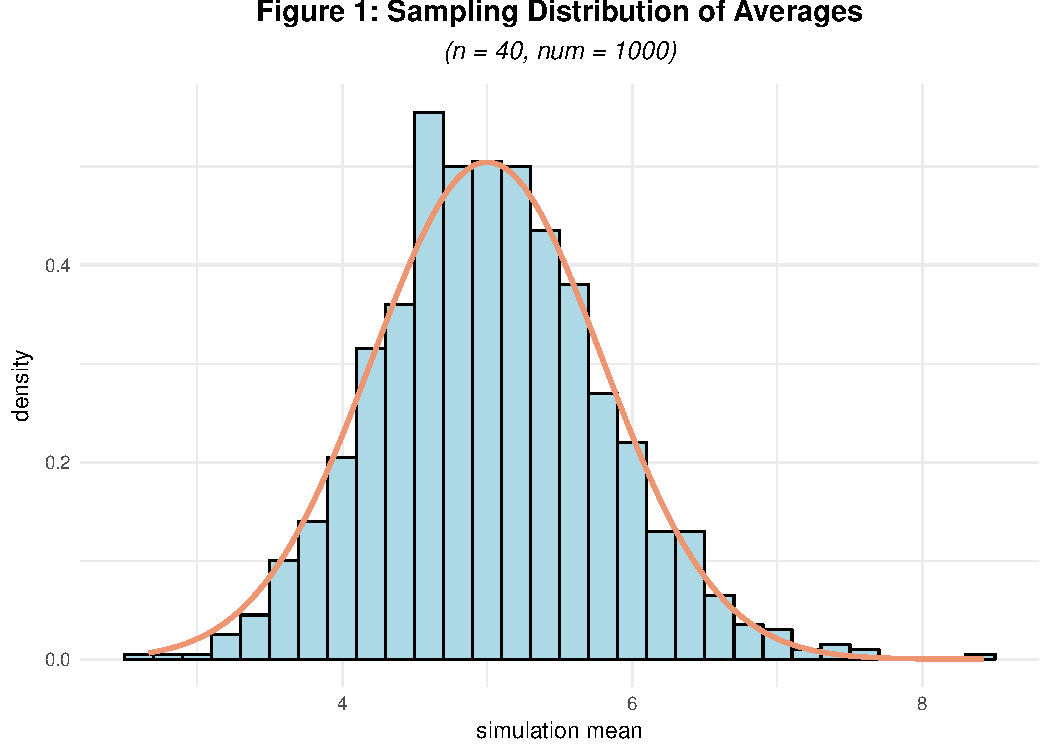
\includegraphics{Final_Project_files/figure-latex/unnamed-chunk-4-1.pdf}

Here the sampling distribution of simulation averages is very similar to
a normal distribution. Use a
\href{https://en.wikipedia.org/wiki/Q\%E2\%80\%93Q_plot}{Q-Q plot} to
confirm our intuitive guess.

\begin{Shaded}
\begin{Highlighting}[]
\KeywordTok{qqnorm}\NormalTok{(mean.simu_exp)}
\KeywordTok{qqline}\NormalTok{(mean.simu_exp, }\DataTypeTok{col =} \DecValTok{2}\NormalTok{)}
\end{Highlighting}
\end{Shaded}

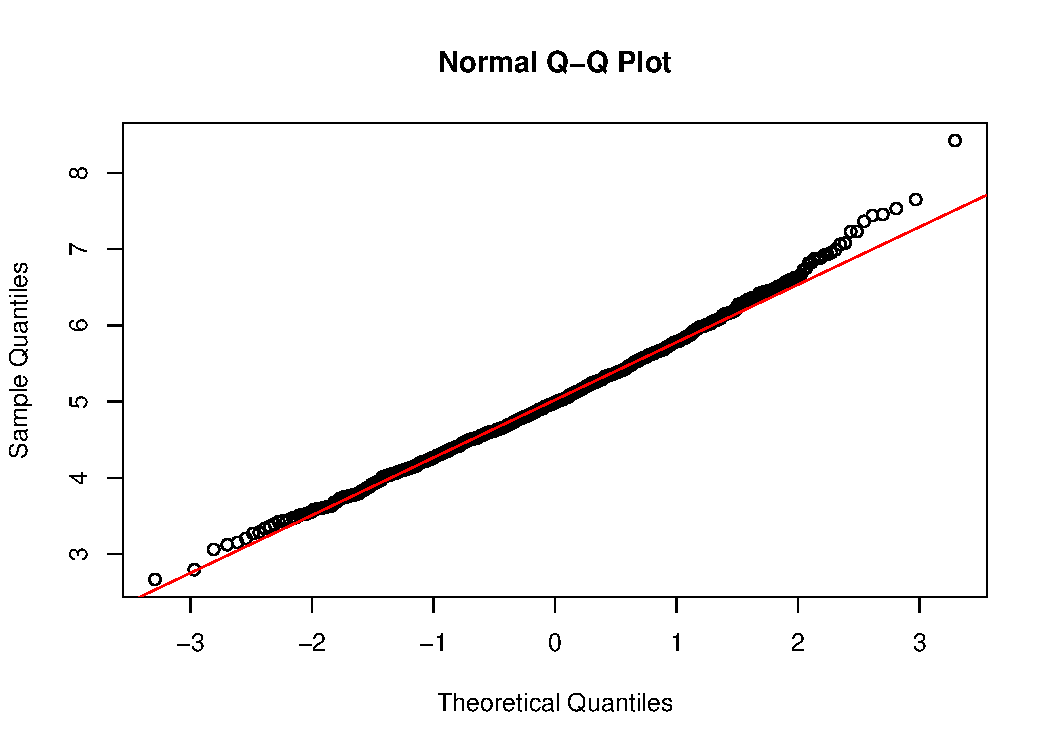
\includegraphics{Final_Project_files/figure-latex/unnamed-chunk-5-1.pdf}

The scatter points converges pretty well to the Q-Q line. Conclude that
CLT works pretty well in this case with 1,000 simulations and 40
simulated samples each.

\newpage

\section{Inferential Data Analysis}\label{inferential-data-analysis}

The following data analysis analyzes the \texttt{ToothGrowth} data set
by comparing the tooth growth by supplement and dose. According to C. I.
Bliss (1952), the response is the length of odontoblasts (cells
responsible for tooth growth) in 60 guinea pigs. Each animal received
one of three dose levels of vitamin C (0.5, 1, and 2 mg/day) by one of
two delivery methods, orange juice or ascorbic acid (a form of vitamin C
and coded as VC). The data set is formated as below:

\begin{longtable}[]{@{}lll@{}}
\caption{Table 1}\tabularnewline
\toprule
Variable & Type & Definition\tabularnewline
\midrule
\endfirsthead
\toprule
Variable & Type & Definition\tabularnewline
\midrule
\endhead
len & numeric & Tooth length\tabularnewline
supp & factor & Supplement type (VC or OJ).\tabularnewline
dose & numeric & Dose in mg/day\tabularnewline
\bottomrule
\end{longtable}

First, load the data and do some exploratory analysis.

\begin{Shaded}
\begin{Highlighting}[]
\KeywordTok{library}\NormalTok{(datasets)}
\KeywordTok{data}\NormalTok{(ToothGrowth)}
\KeywordTok{head}\NormalTok{(ToothGrowth)}
\end{Highlighting}
\end{Shaded}

\begin{verbatim}
##    len supp dose
## 1  4.2   VC  0.5
## 2 11.5   VC  0.5
## 3  7.3   VC  0.5
## 4  5.8   VC  0.5
## 5  6.4   VC  0.5
## 6 10.0   VC  0.5
\end{verbatim}

\newpage

\subsection{Exploratory Data Analysis}\label{exploratory-data-analysis}

\begin{Shaded}
\begin{Highlighting}[]
\KeywordTok{levels}\NormalTok{(ToothGrowth}\OperatorTok{$}\NormalTok{supp) <-}\StringTok{ }\KeywordTok{c}\NormalTok{(}\StringTok{"Orange Juice"}\NormalTok{, }\StringTok{"Ascorbic Acid"}\NormalTok{)}
\KeywordTok{ggplot}\NormalTok{(ToothGrowth, }\KeywordTok{aes}\NormalTok{(}\DataTypeTok{x =} \KeywordTok{factor}\NormalTok{(dose), }\DataTypeTok{y =}\NormalTok{ len)) }\OperatorTok{+}
\StringTok{        }\KeywordTok{facet_grid}\NormalTok{(. }\OperatorTok{~}\StringTok{ }\NormalTok{supp) }\OperatorTok{+}\StringTok{ }
\StringTok{        }\KeywordTok{geom_boxplot}\NormalTok{(}\KeywordTok{aes}\NormalTok{(}\DataTypeTok{fill =}\NormalTok{ supp)) }\OperatorTok{+}
\StringTok{        }\KeywordTok{theme_minimal}\NormalTok{() }\OperatorTok{+}\StringTok{ }
\StringTok{        }\KeywordTok{labs}\NormalTok{(}\DataTypeTok{x=}\StringTok{"dose (mg/day)"}\NormalTok{, }\DataTypeTok{y=}\StringTok{"tooth length"}\NormalTok{) }\OperatorTok{+}
\StringTok{        }\KeywordTok{ggtitle}\NormalTok{(}\StringTok{"Figure 2: Guinea Pig Tooth Length versus Dose by Supplement Type"}\NormalTok{) }\OperatorTok{+}\StringTok{ }
\StringTok{        }\KeywordTok{theme}\NormalTok{(}\DataTypeTok{plot.title =} \KeywordTok{element_text}\NormalTok{(}\DataTypeTok{hjust =} \FloatTok{0.5}\NormalTok{, }\DataTypeTok{vjust =} \DecValTok{3}\NormalTok{, }\DataTypeTok{size =} \DecValTok{14}\NormalTok{, }\DataTypeTok{face =} \StringTok{"bold"}\NormalTok{))}
\end{Highlighting}
\end{Shaded}

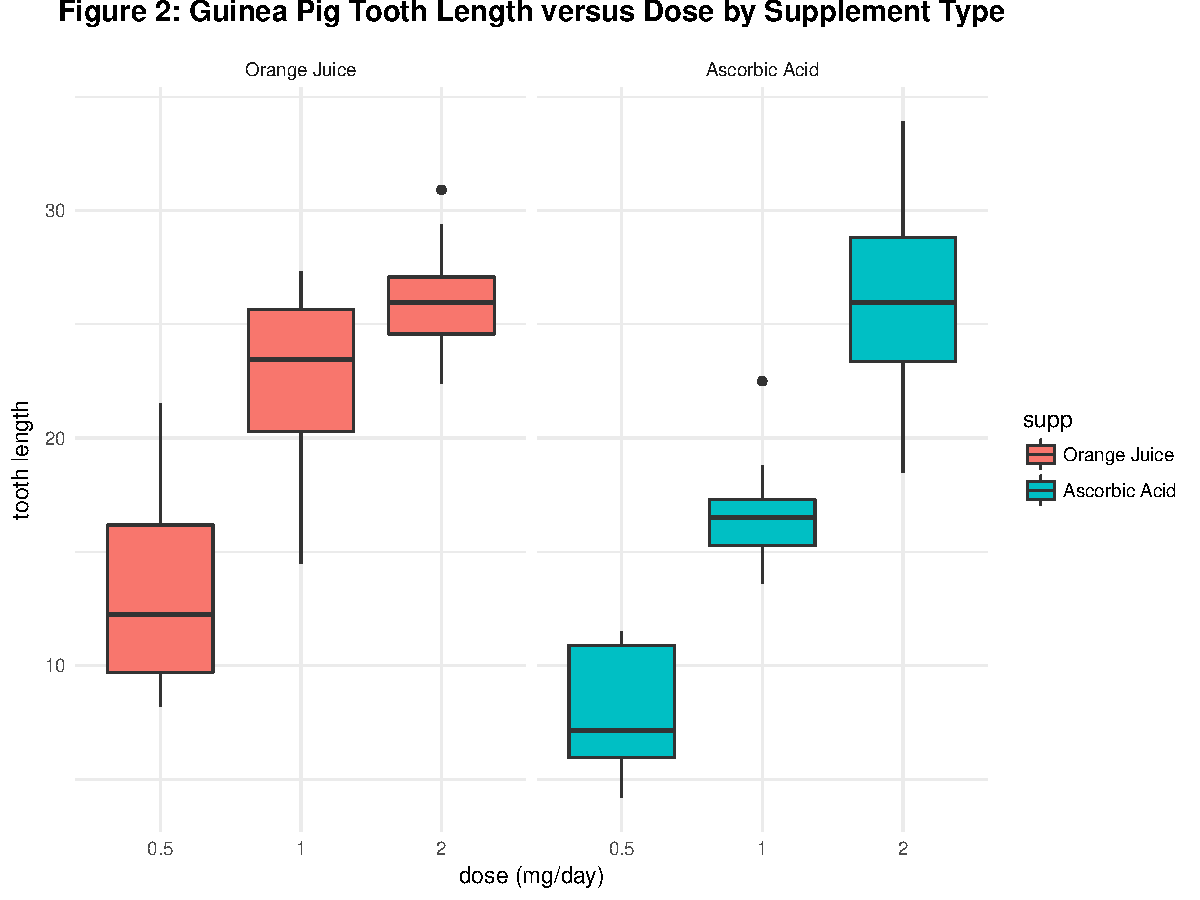
\includegraphics{Final_Project_files/figure-latex/unnamed-chunk-7-1.pdf}

A pattern can be obviously discovered with the panel above, we guess
that tooth length is positively associated with dose and the effect of
dose on tooth length varies across supplement types. There might not be
much difference between average tooth growth of the orange juice group
and the ascorbic acid group on dose level of 2.0 mg.

\newpage

\subsection{Data Summary}\label{data-summary}

\begin{Shaded}
\begin{Highlighting}[]
\KeywordTok{summary}\NormalTok{(ToothGrowth)}
\end{Highlighting}
\end{Shaded}

\begin{verbatim}
##       len                   supp         dose      
##  Min.   : 4.20   Orange Juice :30   Min.   :0.500  
##  1st Qu.:13.07   Ascorbic Acid:30   1st Qu.:0.500  
##  Median :19.25                      Median :1.000  
##  Mean   :18.81                      Mean   :1.167  
##  3rd Qu.:25.27                      3rd Qu.:2.000  
##  Max.   :33.90                      Max.   :2.000
\end{verbatim}

\subsection{Hypothesis Testing}\label{hypothesis-testing}

\subsubsection{Tooth Growth by Supplement via
t-Test}\label{tooth-growth-by-supplement-via-t-test}

Test the hypothesis that ceteris paribus, tooth growth is deifferent
across delivery methods. In other words, use a two tailed t-test under
the significance level of 0.05 with unequal variances across supplement
groups to test the null hypothesis that \(H_0: \mu_1=\mu_2\), where
\(\mu_1\) denotes the mean tooth growth in the \texttt{Orange\ Juice}
group and \(\mu_2\) denotes the mean tooth growth in the
\texttt{Ascorbic\ Acid} group, with an alternative that
\(H_1: \mu_1\ne\mu_2\).

\begin{Shaded}
\begin{Highlighting}[]
\KeywordTok{t.test}\NormalTok{(}\DataTypeTok{data =}\NormalTok{ ToothGrowth, len }\OperatorTok{~}\StringTok{ }\NormalTok{supp, }\DataTypeTok{paired =}\NormalTok{ F, }\DataTypeTok{var.equal =}\NormalTok{ F, }\DataTypeTok{alternative =} \StringTok{"two.sided"}\NormalTok{)}
\end{Highlighting}
\end{Shaded}

\begin{verbatim}
## 
##  Welch Two Sample t-test
## 
## data:  len by supp
## t = 1.9153, df = 55.309, p-value = 0.06063
## alternative hypothesis: true difference in means is not equal to 0
## 95 percent confidence interval:
##  -0.1710156  7.5710156
## sample estimates:
##  mean in group Orange Juice mean in group Ascorbic Acid 
##                    20.66333                    16.96333
\end{verbatim}

Accroding to the test result above, there is no sufficient evidence to
conclude that tooth growth varies across delivery methods, under a
significance level of 0.05.

\subsubsection{Tooth Growth by Dose via
t-Test}\label{tooth-growth-by-dose-via-t-test}

Test the hypothesis that ceteris paribus, tooth growth is deifferent
across dose. Note here although \texttt{dose} is numerical, we should
convert it into factorial as it only takes three values as shown below.

\begin{Shaded}
\begin{Highlighting}[]
\ControlFlowTok{if}\NormalTok{(}\OperatorTok{!}\KeywordTok{require}\NormalTok{(dplyr))\{}\KeywordTok{install.packages}\NormalTok{(}\StringTok{'dplyr'}\NormalTok{)\}}
\KeywordTok{unique}\NormalTok{(ToothGrowth}\OperatorTok{$}\NormalTok{dose)}
\end{Highlighting}
\end{Shaded}

\begin{verbatim}
## [1] 0.5 1.0 2.0
\end{verbatim}

\begin{Shaded}
\begin{Highlighting}[]
\NormalTok{ToothGrowth <-}\StringTok{ }\KeywordTok{mutate}\NormalTok{(ToothGrowth, }\DataTypeTok{dose =} \KeywordTok{as.factor}\NormalTok{(dose))}
\end{Highlighting}
\end{Shaded}

Use a two tailed t-test under the significance level of 0.05 with
unequal variances across dose levels to test the null hypothesis that
\(H_0: \mu_1=\mu_2\), where \(\mu_1\) denotes the mean tooth growth in
dose level of 0.5 and \(\mu_2\) denotes the mean tooth growth in dose
level of 1, with an alternative that \(H_1: \mu_1\ne\mu_2\).

\begin{Shaded}
\begin{Highlighting}[]
\NormalTok{h0.}\DecValTok{1}\NormalTok{ <-}\StringTok{ }\KeywordTok{t.test}\NormalTok{(}\DataTypeTok{data =}\NormalTok{ ToothGrowth[ToothGrowth}\OperatorTok{$}\NormalTok{dose }\OperatorTok\StringTok{ }\KeywordTok{c}\NormalTok{(}\StringTok{"0.5"}\NormalTok{, }\StringTok{"1"}\NormalTok{),], }
\NormalTok{               len }\OperatorTok{~}\StringTok{ }\NormalTok{dose, }\DataTypeTok{paired =}\NormalTok{ F, }\DataTypeTok{var.equal =}\NormalTok{ F, }\DataTypeTok{alternative =} \StringTok{"two.sided"}\NormalTok{)}
\NormalTok{h0.}\DecValTok{1}
\end{Highlighting}
\end{Shaded}

\begin{verbatim}
## 
##  Welch Two Sample t-test
## 
## data:  len by dose
## t = -6.4766, df = 37.986, p-value = 1.268e-07
## alternative hypothesis: true difference in means is not equal to 0
## 95 percent confidence interval:
##  -11.983781  -6.276219
## sample estimates:
## mean in group 0.5   mean in group 1 
##            10.605            19.735
\end{verbatim}

Likewise, use a two tailed t-test under the significance level of 0.05
with unequal variances across dose levels to test the null hypothesis
that \(H_0: \mu_1=\mu_3\), where \(\mu_3\) denotes the mean tooth growth
in dose level of 2, with an alternative that \(H_1: \mu_1\ne\mu_3\).

\begin{Shaded}
\begin{Highlighting}[]
\NormalTok{h0.}\DecValTok{2}\NormalTok{ <-}\StringTok{ }\KeywordTok{t.test}\NormalTok{(}\DataTypeTok{data =}\NormalTok{ ToothGrowth[ToothGrowth}\OperatorTok{$}\NormalTok{dose }\OperatorTok\StringTok{ }\KeywordTok{c}\NormalTok{(}\StringTok{"0.5"}\NormalTok{, }\StringTok{"2"}\NormalTok{),], }
\NormalTok{               len }\OperatorTok{~}\StringTok{ }\NormalTok{dose, }\DataTypeTok{paired =}\NormalTok{ F, }\DataTypeTok{var.equal =}\NormalTok{ F, }\DataTypeTok{alternative =} \StringTok{"two.sided"}\NormalTok{)}
\NormalTok{h0.}\DecValTok{2}
\end{Highlighting}
\end{Shaded}

\begin{verbatim}
## 
##  Welch Two Sample t-test
## 
## data:  len by dose
## t = -11.799, df = 36.883, p-value = 4.398e-14
## alternative hypothesis: true difference in means is not equal to 0
## 95 percent confidence interval:
##  -18.15617 -12.83383
## sample estimates:
## mean in group 0.5   mean in group 2 
##            10.605            26.100
\end{verbatim}

Further, use a two tailed t-test under the significance level of 0.05
with unequal variances across dose levels to test the null hypothesis
that \(H_0: \mu_2=\mu_3\), with an alternative that
\(H_1: \mu_2\ne\mu_3\).

\begin{Shaded}
\begin{Highlighting}[]
\NormalTok{h0.}\DecValTok{3}\NormalTok{ <-}\StringTok{ }\KeywordTok{t.test}\NormalTok{(}\DataTypeTok{data =}\NormalTok{ ToothGrowth[ToothGrowth}\OperatorTok{$}\NormalTok{dose }\OperatorTok\StringTok{ }\KeywordTok{c}\NormalTok{(}\StringTok{"1"}\NormalTok{, }\StringTok{"2"}\NormalTok{),], }
\NormalTok{               len }\OperatorTok{~}\StringTok{ }\NormalTok{dose, }\DataTypeTok{paired =}\NormalTok{ F, }\DataTypeTok{var.equal =}\NormalTok{ F, }\DataTypeTok{alternative =} \StringTok{"two.sided"}\NormalTok{)}
\NormalTok{h0.}\DecValTok{3}
\end{Highlighting}
\end{Shaded}

\begin{verbatim}
## 
##  Welch Two Sample t-test
## 
## data:  len by dose
## t = -4.9005, df = 37.101, p-value = 1.906e-05
## alternative hypothesis: true difference in means is not equal to 0
## 95 percent confidence interval:
##  -8.996481 -3.733519
## sample estimates:
## mean in group 1 mean in group 2 
##          19.735          26.100
\end{verbatim}

\newpage

Print a summary of the tested hypothesis, corresponding t-statistic,
p-value and confidence interval.

\begin{verbatim}
##   Tested.Hypothesis t.Statistic p.value   Confidence.Interval
## 1   0.5 mg - 1.0 mg      -6.477       0  [ -11.984 , -6.276 ]
## 2   0.5 mg - 2.0 mg     -11.799       0 [ -18.156 , -12.834 ]
## 3   1.0 mg - 2.0 mg      -4.900       0   [ -8.996 , -3.734 ]
\end{verbatim}

According to the test results above, we can reject the null hypotheses
and conclude that ceteris paribus, average tooth growth is different
across levels of dose, under a significance level of 0.05. As all the
confidence intervals lies below 0, we expect a positive relationship.

\subsubsection{Tooth Growth by Supplement and Dose via
t-Test}\label{tooth-growth-by-supplement-and-dose-via-t-test}

It seems too early to conclude that tooth growth is independent from
supplement (recall the pattern we observed in figure 2). Further test
the significance of supplement effects conditioned on dose, i.e.~take
both IVs into consideration. In my analysis, the effects of supplement
conditioned on dose were tested.

Use a two tailed t-test under the significance level of 0.05 with
unequal variances across supplement groups \textbf{conditioned on dose
level of 0.5 mg} to test the null hypothesis that \(H_0: \mu_1=\mu_2\),
where \(\mu_1\) denotes the mean tooth growth in the
\texttt{Orange\ Juice} group and \(\mu_2\) denotes the mean tooth growth
in the \texttt{Ascorbic\ Acid} group on a dose level of 0.5 mg, with an
alternative that \(H_1: \mu_1\ne\mu_2\).

\begin{Shaded}
\begin{Highlighting}[]
\NormalTok{h1.}\DecValTok{1}\NormalTok{ <-}\StringTok{ }\KeywordTok{t.test}\NormalTok{(}\DataTypeTok{data =}\NormalTok{ ToothGrowth[ToothGrowth}\OperatorTok{$}\NormalTok{dose }\OperatorTok\StringTok{ }\KeywordTok{c}\NormalTok{(}\StringTok{"0.5"}\NormalTok{),], }
\NormalTok{               len }\OperatorTok{~}\StringTok{ }\NormalTok{supp, }\DataTypeTok{paired =}\NormalTok{ F, }\DataTypeTok{var.equal =}\NormalTok{ F, }\DataTypeTok{alternative =} \StringTok{"two.sided"}\NormalTok{)}
\NormalTok{h1.}\DecValTok{1}
\end{Highlighting}
\end{Shaded}

\begin{verbatim}
## 
##  Welch Two Sample t-test
## 
## data:  len by supp
## t = 3.1697, df = 14.969, p-value = 0.006359
## alternative hypothesis: true difference in means is not equal to 0
## 95 percent confidence interval:
##  1.719057 8.780943
## sample estimates:
##  mean in group Orange Juice mean in group Ascorbic Acid 
##                       13.23                        7.98
\end{verbatim}

Likewise, use a two tailed t-test under the significance level of 0.05
with unequal variances across supplement groups \textbf{conditioned on
dose level of 1.0 mg} to test the null hypothesis that
\(H_0: \mu_1=\mu_2\),where \(\mu_1\) denotes the mean tooth growth in
the \texttt{Orange\ Juice} group and \(\mu_2\) denotes the mean tooth
growth in the \texttt{Ascorbic\ Acid} group on a dose level of 1.0 mg,
with an alternative that \(H_1: \mu_1\ne\mu_2\).

\begin{Shaded}
\begin{Highlighting}[]
\NormalTok{h1.}\DecValTok{2}\NormalTok{ <-}\StringTok{ }\KeywordTok{t.test}\NormalTok{(}\DataTypeTok{data =}\NormalTok{ ToothGrowth[ToothGrowth}\OperatorTok{$}\NormalTok{dose }\OperatorTok\StringTok{ }\KeywordTok{c}\NormalTok{(}\StringTok{"1"}\NormalTok{),],}
\NormalTok{               len }\OperatorTok{~}\StringTok{ }\NormalTok{supp, }\DataTypeTok{paired =}\NormalTok{ F, }\DataTypeTok{var.equal =}\NormalTok{ F, }\DataTypeTok{alternative =} \StringTok{"two.sided"}\NormalTok{)}
\NormalTok{h1.}\DecValTok{2}
\end{Highlighting}
\end{Shaded}

\begin{verbatim}
## 
##  Welch Two Sample t-test
## 
## data:  len by supp
## t = 4.0328, df = 15.358, p-value = 0.001038
## alternative hypothesis: true difference in means is not equal to 0
## 95 percent confidence interval:
##  2.802148 9.057852
## sample estimates:
##  mean in group Orange Juice mean in group Ascorbic Acid 
##                       22.70                       16.77
\end{verbatim}

Last, use a two tailed t-test under the significance level of 0.05 with
unequal variances across supplement groups \textbf{conditioned on dose
level of 2.0 mg} to test the null hypothesis that \(H_0: \mu_1=\mu_2\),
where \(\mu_1\) denotes the mean tooth growth in the
\texttt{Orange\ Juice} group and \(\mu_2\) denotes the mean tooth growth
in the \texttt{Ascorbic\ Acid} group on a dose level of 2.0 mg, with an
alternative that \(H_1: \mu_1\ne\mu_2\).

\begin{Shaded}
\begin{Highlighting}[]
\NormalTok{h1.}\DecValTok{3}\NormalTok{ <-}\StringTok{ }\KeywordTok{t.test}\NormalTok{(}\DataTypeTok{data =}\NormalTok{ ToothGrowth[ToothGrowth}\OperatorTok{$}\NormalTok{dose }\OperatorTok\StringTok{ }\KeywordTok{c}\NormalTok{(}\StringTok{"2"}\NormalTok{),], }
\NormalTok{               len }\OperatorTok{~}\StringTok{ }\NormalTok{supp, }\DataTypeTok{paired =}\NormalTok{ F, }\DataTypeTok{var.equal =}\NormalTok{ F, }\DataTypeTok{alternative =} \StringTok{"two.sided"}\NormalTok{)}
\NormalTok{h1.}\DecValTok{3}
\end{Highlighting}
\end{Shaded}

\begin{verbatim}
## 
##  Welch Two Sample t-test
## 
## data:  len by supp
## t = -0.046136, df = 14.04, p-value = 0.9639
## alternative hypothesis: true difference in means is not equal to 0
## 95 percent confidence interval:
##  -3.79807  3.63807
## sample estimates:
##  mean in group Orange Juice mean in group Ascorbic Acid 
##                       26.06                       26.14
\end{verbatim}

Further, print a summary table of the tested hypothesis, corresponding
t-statistic, p-value and confidence interval.

\begin{verbatim}
##   Conditioned.Dose t.Statistic p.value Confidence.Interval
## 1           0.5 mg       3.170   0.006   [ 1.719 , 8.781 ]
## 2           1.0 mg       4.033   0.001   [ 2.802 , 9.058 ]
## 3           2.0 mg      -0.046   0.964  [ -3.798 , 3.638 ]
\end{verbatim}

According to the test results above, \textbf{conditioned on dose levels
of 0.5 mg and 1.0 mg}, we can reject the null hypotheses and conclude
that average tooth growth is different across types of supplement, under
a significance level of 0.05. Here all the confidence intervals are
above 0, we expect a positive effect of orange juice over ascorbic acid
conditioned on a dose level of 0.5 mg or 1.0 mg. When the dose level
equals 2.0 mg, the difference in average tooth growth is no longer
significant.

\subsection{Conclusions and
Assumptions}\label{conclusions-and-assumptions}

Based on the simple inferential data analysis above, we conclude that:

\begin{itemize}
\tightlist
\item
  There is no strong evidence indicating that tooth length varies based
  on delivery methods independent of dose level;
\item
  However, there is significant evidence showing that it varies when the
  dose level is contolled at either 0.5mg or 1.0 mg, under a
  significance level of 0.05, and expect a postive effect of orange
  juice over ascorbic acid as a better delivery method;
\item
  We are 95\% confident that tooth length varies across levels of dose
  and expect a positive relationship between tooth growth and dosage
\end{itemize}

The underlying assumptions include:

\begin{itemize}
\tightlist
\item
  Populations of guinea pigs were independent;
\item
  Variances across groups are NOT equal, which is rather conservative
\end{itemize}


\end{document}
